\documentclass[tikz]{standalone}
\usepackage{xcolor}
\definecolor{bg}{HTML}{171D2B}
\definecolor{aksen}{HTML}{F7B538}
\begin{document}
\pagecolor{bg}
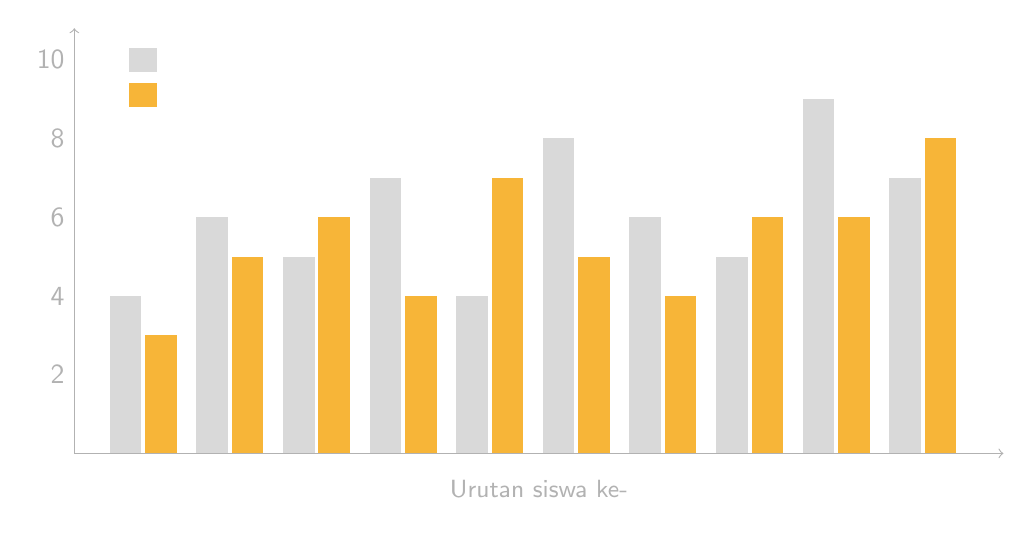
\begin{tikzpicture}[x=1cm,y=1cm,text=white,font=\sffamily]
% koordinat kelas 7A dan 7B
\def\A{4,6,5,7,4,8,6,5,9,7,5,6,8,4,7,6,5,8,6,7}
\def\B{3,5,6,4,7,5,4,6,6,8,5,4,7,6,5,7,4,6,5,5}
% sumbu
\draw[white!70!black,->] (-0.4,0) -- (11.4,0);
\draw[white!70!black,->] (-0.4,0) -- (-0.4,5.4);
% grid ringan
\foreach \y in {1,...,5} \draw[white!20] (0,\y) -- (11.2,\y);
\foreach \y/\t in {1/2,2/4,3/6,4/8,5/10} \node[left,white!70!black] at (-0.4,\y) {\t};
% pasangan batang: putih (7A), aksen (7B)
\foreach \i in {0,...,9} {
  \pgfmathsetmacro{\na}{{\A}[\i]/2}
  \pgfmathsetmacro{\nb}{{\B}[\i]/2}
  \pgfmathsetmacro{\x}{\i*1.1}
  \fill[white!85!black]   (\x+0.05,0) rectangle (\x+0.45,\na);
  \fill[aksen]            (\x+0.50,0) rectangle (\x+0.90,\nb);
}
% legenda
\fill[white!85!black] (0.3,4.85) rectangle (0.65,5.15);
\node[anchor=west,font=\sffamily\small] at (0.75,5.0) {Kelas 7A};
\fill[aksen] (0.3,4.4) rectangle (0.65,4.7);
\node[anchor=west,font=\sffamily\small] at (0.75,4.55) {Kelas 7B};
\node[font=\sffamily\small,white!70!black] at (5.5,-0.45) {Urutan siswa ke-};
\end{tikzpicture}
\end{document}
